%%%------------------------------------------------------------------
%%% Filename: l2tabufr.tex
%%% Author: Marc Ensenbach <Marc.Ensenbach@post.rwth-aachen.de>
%%% Orig. Author: Mark Trettin <Mark.Trettin@gmx.de>
%%% Created: 07 Mär 2005 13:36:50
%%% Last Modif.: 20 Sep 2011
%%% Version: 2.3
%%%
%%% Copyright (C) 2005 by Mark Trettin
%%% Copyright (C) 2010 by Marc Ensenbach
%%%%%%%%%%%%%%%%%%%%%%%%%%%%%%%
%%% Traduction française : Bernard Alfonsi, à partir de la traduction de la version 1.7
%%% par le TeXnicien de surface, de la version allemande 2.3 et de sa traduction italienne.

%%% Créée le 12-7-2013
%%%------------------------------------------------------------------

\documentclass[fontsize=11pt, paper=a4, pagesize, captions=tableheading, numbers=enddot, toc=graduated, footnotes=multiple]{scrartcl}%
%--------------- Configuration de base (français, 8bit) ----------------
\usepackage[utf8]{inputenc} % Saisie directe des umlauts, etc.
\usepackage[T1]{fontenc} % Polices T1
\usepackage{numprint}
\usepackage[autostyle, french=guillemets,german=guillemets]{csquotes}
\MakeAutoQuote{«}{»}% Autoquotes pour csquotes.sty
\usepackage{comment}
% -------------------------------- Polices ---------------------------------
\usepackage[scaled=.88]{beramono} % Bera-Monospace
\usepackage[scaled=.86]{berasans} % Bera Sans-Serif
\usepackage[osf]{mathpazo} % Palatino est la police par défaut
\linespread{1.05}\selectfont % Palatino requiert un interlignage plus grand
%%% Ce qui suit n’est pas très propre, mais ça marche (ici : Palatino)
\providecommand{\lining}{\fontfamily{ppl}\selectfont}
\providecommand{\oldstyle}{\fontfamily{fplj}\selectfont}
\DeclareTextFontCommand{\textln}{\lining}
\DeclareTextFontCommand{\textos}{\oldstyle}

%------------ Extensions supplémentaires (graphiques, tableaux) ---------------
\usepackage{xspace} % espaces automatiques après les macros
\usepackage{booktabs,array} % tableaux plus avenants
\usepackage[french]{varioref} % modifié pour la version publique,
                                % car la version actuelle de fancy, et
                                % varioref ne fonctionnent pas ensemble
                                % (toujours pas ?!)

\usepackage{textcomp} % Symboles supplémentaires
\usepackage[nofancy]{rcsinfo} % Données RCSdans les titres
\usepackage{varwidth} % Für die Ersetze-Umgebungen,
\usepackage{calc} % Pour calculer
\usepackage{amsmath, amssymb}
\usepackage{graphicx}
%--------------------------- Mise en forme ---------------------------
%%% Captions
\addtokomafont{pagehead}{\small\itshape}
\addtokomafont{sectioning}{\rmfamily}
\addtokomafont{caption}{\footnotesize\itshape}
\addtokomafont{captionlabel}{\scshape}% modifié par B. A.
\addtokomafont{descriptionlabel}{\rmfamily}
\setcapindent{1em}
\deffootnote{2.25em}{1.75em}{\thefootnotemark\enspace}
%%% Titres
\reversemarginpar
\renewcommand*{\othersectionlevelsformat}[1]{%
  \makebox[0pt][r]{\csname the#1\endcsname\autodot\enskip}}
\renewcommand*{\captionformat}{~--~}%%ajout de B. A.
% --------------------------------- Couleurs-----------------------------------
\usepackage{color}
\definecolor{grau}{gray}{0.45}
\definecolor{rot}{rgb}{0.75,0.00,0.00}
\definecolor{blau}{rgb}{0.16,0.24,0.64}
\definecolor{gruen}{rgb}{0.18,0.58,0.08}
\definecolor{linkcolor}{rgb}{0,0,0.42}

%--------------------------- Options PDF ---------------------------
\ifpdfoutput{% %Requiert les classes KOMA-Script
 \usepackage{hyperref} % réglages de hyperref pour pdf[pagebackref]
 \hypersetup{%
 pdfauthor={(c) 2003, 2004, 2005, 2006, 2007 Mark Trettin,
2009, 2010, 2011 Marc Ensenbach},%
 pdftitle={ Liste des péchés des utilisateurs de LaTeX 2e ou Commandes et extensions obsolètes, et autres erreurs},%
 pdfsubject={Quelques conseils à propos de LaTeX 2e},%
 bookmarksopen=true,%
 %backref=true,
 linktocpage=true,
 urlcolor=linkcolor,
 citecolor=linkcolor,
 linkcolor=linkcolor,
 colorlinks=true,
 }
 \usepackage{microtype}
%% Ultérieurement, il nous faudra la possibilité de désactiver la microtypographie%
%% pour les exemples qui démontreront le comportement standard de LaTeX [Marc]
 \SetExpansion[context=slbsp, factor=0]{encoding={OT1, T1, TS1}}{}
  \newcommand{\EMail}[1]{\href{mailto:#1?Subject=[l2tabu.pdf]}{courriel : \texttt{#1}}}
  \newcommand{\News}[1]{\href{news:#1}{\texttt{#1}}}
%% Cette définition est fumeuse, il faudra que j’y réfléchisse de nouveau. :-(
%% Je ferai cela plus tard [Marc]
  \newcommand{\MID}[2]{\href{http://groups.google.com/groups?as_umsgid=#1}%
    {Message-ID: \texttt{<#2>}}}
%--------------------------- Options PS----------------------------
}{%
    \usepackage{hyperref}
    \newcommand{\EMail}[1]{\href{mailto:#1}{\texttt{#1}}}
    \newcommand{\News}[1]{\href{news:#1}{\texttt{#1}}}
    \newcommand{\MID}[2]{\href{M-ID: <#1>}{Message-ID: \texttt{<#2>}}}
  }
%-------------------------- Nouvelles commandes --------------------------
%%% Volées à scrguide ;-)
\DeclareRobustCommand*{\Macro}[1]{\mbox{\texttt{\char`\\#1}}}
\DeclareRobustCommand*{\LMacro}[2]{\mbox{\texttt{\char`\\#1\{#2\}}}}
\DeclareRobustCommand*{\GMacro}[2]{\mbox{\texttt{\{\char`\\#1\ #2\}}}}

%%% DANTE
\providecommand{\CTANserver}{ftp.dante.de}
%%% Fait de CTAN:// un alias de ftp://\CTANserver/tex-archive/
\makeatletter
\def\url@#1{\expandafter\url@@#1\@nil}
\def\url@@#1://#2\@nil{%
  \def\@tempa{#1}\def\@tempb{CTAN}\ifx\@tempa\@tempb
    \hyper@linkurl{\Hurl{#1:#2}}{ftp://\CTANserver/tex-archive/#2}%
  \else
    \hyper@linkurl{\Hurl{#1://#2}}{#1://#2}%
  \fi
}
\makeatother

%%% Logo XeLaTeX (\XeTeX adapté du logo dtk)
\newcommand{\XeLaTeX}{\smash{X\kern-.1em\lower.5ex\hbox{\reflectbox{E}}\kern-.07em\LaTeX}}

%%% de moi pour \dots
\pdfstringdefDisableCommands{%
  \edef\dots{\string...}%
}

%%% Hack tout à fait rudimentaire pour qu’une url tienne sur une seule ligne
%%% *sans* espacement supplémentaire
\newcommand{\biburl}[1]{\hfill\\URL:~\url{#1}}

%%% Commandes
\newcommand{\zB}{zum Beispiel\xspace}%raccourci associé à l’allemand : par exemple
\newcommand{\ZB}{Zum Beispiel\xspace}%idem : Par exemple
\newcommand{\bzw}{beziehungsweise\xspace}%idem : respectivement
%%% documentation : SansSerif
\newcommand{\Doku}[1]{\textsf{#1}\xspace}
%%% extension , classe, style bibliographique : SansSerif
\newcommand{\Paket}[1]{\textsf{#1.sty}\xspace}
\newcommand{\PakeH}[1]{#1.sty\xspace}
\newcommand{\Klasse}[1]{\textsf{#1.cls}\xspace}
\newcommand{\KlassH}[1]{#1.cls\xspace}
\newcommand{\Bst}[1]{\textsf{#1.bst}\xspace}
\newcommand{\BstH}[1]{#1.bst\xspace}
%%% Options : SansSerif
\newcommand{\Option}[1]{\textsf{#1}\xspace}

\newcommand{\TB}{\textbackslash}

%%% Cela ne me plaît plus. Suggestion ?
%%% Non. J’y réfléchirai plus tard. [Marc]
\newcommand{\schlecht}[1][!]{\marginline{\texttt{#1}}}

%%%% Ambiente "NON\dots MA"
%\newenvironment{Ers}[1][\linewidth]{%
% \par\smallskip\noindent\textcolor{rot}{\textbf{\textsf{NON:}}\marginline{$
% \triangleright$}}~\rahmenpr[#1]}%
%{\endrahmenpr\hfill}
%\newenvironment{Dur}[1][\linewidth]{%
%\noindent\textcolor{gruen}{\textbf{\textsf{MA:}}}~\rahmenpg[#1]}%
%{\endrahmenpg\noindent}
%
%% Ambiente "Schecht"
%\newenvironment{Schlecht}[1][\linewidth]{%
% \par\smallskip\rahmenpr[#1]}%
%{\endrahmenpr\par\noindent}
%
%% Ambienti "rahmenlength" e "rahmenpg"
%\newsavebox{\rahmenbox}
%\setlength{\fboxrule}{0.6pt}
%\newlength{\rahmenlength}
%\newenvironment{rahmenpr}[1][\linewidth]{%
% \setlength{\rahmenlength}{#1-2\fboxsep-2\fboxrule}%
% \begin{lrbox}{\rahmenbox}\begin{varwidth}[t]{\rahmenlength}}
% {\end{varwidth}\end{lrbox}\noindent\fcolorbox{rot}{white}{\usebox{\rahmenbox}}\vspace*{.5ex}}
%\newenvironment{rahmenpg}[1][\linewidth]{%
% \setlength{\rahmenlength}{#1-2\fboxsep-2\fboxrule}%
% \begin{lrbox}{\rahmenbox}\begin{varwidth}[t]{\rahmenlength}}
% {\end{varwidth}\end{lrbox}\noindent\fcolorbox{gruen}{white}{\usebox{\rahmenbox}}\vspace*{.5ex}}

%%%Environnement « Remplacez »
\newenvironment{Ers}[1][\linewidth]{%
  \par\bigskip\noindent\marginline{\textcolor{gruen}{\boldmath $\triangleright$}}\begin{tabular}[t]{@{}p{0.5\textwidth}@{}}\textcolor{rot}{\textbf{\textsf{Remplacez~:}}%
}\\[2pt] \rahmenpr[#1]}%
{\endrahmenpr\end{tabular}}
% % «... par : »
\newenvironment{Dur}[1][0.5\textwidth]{%
\noindent\begin{tabular}[t]{@{}p{0.5\textwidth - 0.5em}@{}}\textcolor{gruen}{\textbf{\textsf{par~:}}}\\[2pt]\rahmenpg[#1]}%
{\endrahmenpg\end{tabular}\smallskip\noindent}

%%% Environnement Schlecht (« mauvais »)
\newenvironment{Schlecht}[1][\linewidth]{%
  \par\medskip\rahmenpr[#1]}%
{\endrahmenpr\par\noindent}

%%% Environnements « rahmenpr » et « rahmenpg »
\newsavebox{\rahmenbox}
\setlength{\fboxrule}{0.6pt}
\setlength{\fboxsep}{1ex} %% ajouté par moi — au lieu de 3 pt
\newlength{\rahmenlength}

\newenvironment{rahmenpr}[1][0.5\linewidth]{%
  \setlength{\rahmenlength}{#1-2\fboxsep-2\fboxrule}%
  \begin{lrbox}{\rahmenbox}\begin{varwidth}[t]{\rahmenlength}}
    {\end{varwidth}\end{lrbox}\noindent\fcolorbox{rot}{white}{\usebox{\rahmenbox}}\vspace*{.5ex}}

\newenvironment{rahmenpg}[1][0.5\linewidth]{%
  \setlength{\rahmenlength}{#1-2\fboxsep-2\fboxrule}%
  \begin{lrbox}{\rahmenbox}\begin{varwidth}[t]{\rahmenlength}}
    {\end{varwidth}\end{lrbox}\noindent\fcolorbox{gruen}{white}{\usebox{\rahmenbox}}\vspace*{.5ex}}

% Environnement description : espacement un peu plus petit entre deux items
\newenvironment{description*}{%
  \description%
    \setlength{\itemsep}{0pt}}%
  {\enddescription}
\newsavebox{\Quelle}

% Environnement « Exemple de code »
\newenvironment{bspcode}[1]{%
  \sbox{\Quelle}{\footnotesize Source : #1}
  \center
  \rule{\linewidth}{1.5pt}
}{%
  \rule{\linewidth}{1.5pt}
  \usebox{\Quelle}
  \endcenter%
}

%------------------- Définitions de colonnes pour tableaux--------------------
% Requiert l’extension array
\newcolumntype{F}{>{\footnotesize}l}%% N dans l’original, mais déjà pris par numprint (B. A.)

%%%%%%%%%%%%%%%%%%%%%%%%%%%%%%%%%%%%%%%%%%%%%%%%%%%%%%%%%%%%%%%%%%%%%%
\usepackage[ngerman, frenchb]{babel} % Motifs de césure français
\frenchbsetup{ReduceListSpacing = true, IndentFirst = false, }%
\addto{\captionsfrench}{\renewcommand*{\pagename}{p.}\renewcommand{\figurename}{Fig.}}
%%% ------------- macros pour la traduction française -------------
\newcommand{\NDT}{[T\textsubscript{dS}].} % ça c'est moi ;)
\newcommand{\PakeT}[1]{\textsf{\textsl{#1.sty}}}%
\renewcommand{\thefootnote}{\lining\arabic{footnote}}
\renewcommand{\labelenumi}{\lining\arabic{enumi}.}
\renewcommand{\thesection}{\lining\arabic{section}}

\def\reftextfaraway#1{p.~\pageref{#1}}% redéfinition de varioref
%%%-----------– extensions supplémentaires -------------------
\usepackage[para]{threeparttable}
\renewcommand{\TPTtagStyle}{\textit}
\usepackage[shortlabels]{enumitem}

\makeatletter
\newcommand{\oldstyleroman}[1]{\expandafter\@oldstyleroman#1\@nil}
\def\@oldstyleroman#1#2\@nil{%
 \ifcat$\detokenize{#2}$%
 \expandafter\@firstoftwo
 \else
 \expandafter\@secondoftwo
 \fi
 {\if#1ij\else#1\fi}% si #2 est vide
 {#1\@oldstyleroman#2\@nil}% si #2 n'est pas vide
}
\def\scroman#1{\expandafter\@scroman\csname c@#1\endcsname}
\def\@scroman#1{{\scshape\romannumeral #1}}
\def\osroman#1{\expandafter\@osroman\csname c@#1\endcsname}
\def\@osroman#1{\oldstyleroman{\romannumeral #1}}
%%\def\osroman#1{\expandafter\@osroman\csname c@#1\endcsname}
%%\def\@osroman#1{{\shortromannumeral #1}}
\makeatother
%
%\usepackage{modroman}

\raggedbottom

%----------------------- début du document -----------------------

\begin{document}
%\begin{Form}\end{Form}
\pagestyle{headings}
%%% RCS Info for version control
\rcsInfo $Id: l2tabu.tex,v 2.3 2011/09/20 09:18:00 yvon Exp $
%%%----------------------------- Page de titre ----------------------------

\pagenumbering{osroman}
\begin{titlepage}
\pdfbookmark[1]{Page de titre}{tit}
\begin{flushleft}
    \noindent
  \rule{\linewidth}{1pt}%
  \vspace{2\baselineskip}
  {\LARGE\bfseries
  Liste des péchés des utilisateurs de \LaTeXe\\[1ex]
    \large
   \quad ou\\[0.5\baselineskip]
         Commandes et extensions obsolètes, et autres erreurs}\\
  \vspace{2\baselineskip}
  \noindent
  \rule{\linewidth}{1pt}%
\end{flushleft}
  \vspace{\baselineskip}
\begin{flushright}
  \textit{Marc Ensenbach, Mark Trettin}\\
  \EMail{Marc.Ensenbach@post.rwth-aachen.de}\\[1.5\baselineskip]
  Version \rcsInfoRevision\ du \rcsInfoLongDate\\[1.5\baselineskip]
  {\footnotesize Traduction française de Bernard Alfonsi\\
  \EMail{bernard.alfonsi@free.fr}}\\[4\baselineskip]
\end{flushright}
  \vspace{\baselineskip}
  \begin{center}
    \let\footnoterule\relax
    \begin{minipage}{.9\linewidth}
      \small
      \begin{center}
        \textbf{Résumé}
      \end{center}
      \noindent

%%%%%%%%%%%%% Traduction de l’introduction italienne %%%%%%%%%%%%%%%
% Elle correspond dans une large mesure à la version originale allemande la plus récente et, hormis des modifications et ajouts mineurs, ne s’en écarte de façon significative que dans la section \vref{sec:die-verwendung-von}, qui a été complètement récrite. Les parties modifiées ont été indiquées en note, à la demande explicite de l’auteur. Le traducteur, qui s’est servi des remarques soulevées à ce sujet par les membres du \GuIT, désire remercier ici tout particulièrement Claudio Beccari et Tommaso Gordini. Enfin, ma reconnaissance va à l’auteur, Marc Ensenbach, qui a lu avec soin cette version italienne et fait des remarques supplémentaires.
%%%%%%%%%%%%% Fin de l’\/introduction italienne %%%%%%%%%%%%%%%%%%%
 \emph{Ceci est la version française de «l2tabu». — }
La rédaction de ce bref aperçu a été suscitée par une discussion dans le newsgroup \TeX{} de langue allemande\footnote{\News{de.comp.text.tex}}, où revenaient de façon récurrente des extensions et des commandes obsolètes ou «mauvaises».

Nous essayons dans cet article de montrer les erreurs les plus communes et de proposer des solutions différentes. Cet article n’entend pas remplacer des introductions comme \Doku{l2kurz}~\cite{l2kurz-12} ni \Doku{De-TeX-FAQ}\footnote{\url{http://projekte.dante.de/DanteFAQ/WebHome}}, ni \Doku{The UK \TeX{} FAQ}~\cite{ukfaq-13}, mais offrir un simple aperçu.

Nous serions reconnaissants de vos suggestions, améliorations et commentaires.
    \end{minipage}
  \end{center}
  \vfill
\end{titlepage}
%------------------------ Fin de la page de titre ----------------------------

%%%%%%%%%%%%%%%%%%%%%%%%%%%%%%%Copyright
{\setlength{\parindent}{0pt}
Copyright \copyright{} 2003--2007 by Mark Trettin, 2009--2011 by Marc Ensenbach. \medskip

This material may be distributed only subject to the terms and conditions set forth in the \emph{Open Publication License}, v1.0 or later (the latest version is presently available at \url{http://www.opencontent.org/openpub/}).
\medskip

Cette documentation peut être distribuée seulement aux termes et conditions de l’\emph{Open Publication License}, v1.0 ou postérieure (la version la plus récente est actuellement disponible à l’adresse : \url{http://www.opencontent.org/openpub/}).
\medskip

Les noms de \emph{software} et de \emph{hardware} mentionnés dans cet article sont pour la plupart, des marques déposées, soumises, comme telles, aux dispositions légales.
\vfill

Nous remercions : \\
Ralf Angeli,
Christoph Bier,
Christian Faulhammer,
Jürgen Fenn\footnote{Traduction anglaise : \url{CTAN://info/l2tabu/english/l2tabuen.pdf}},
Ulrike Fischer,
Ralf Heckmann,
Yvon Henel\footnote{Traduction française : \url{CTAN://info/l2tabu/french/l2tabufr.pdf}},
Yvonne Hoffmüller,
David Kastrup,
Markus Kohm,
Thomas Lotze,
Gonzalo Medina Arellano\footnote{Traduction espagnole : \url{CTAN://info/l2tabu/spanish/l2tabues.pdf}},
Frank Mittelbach,
Heiko Oberdiek,
Mauro Sacchetto\footnote{Traduction italienne : \url{CTAN://info/l2tabu/italian/l2tabuit.pdf}},
Walter Schmidt,
Uwe Siart,
Stefan Stoll,
Knut Wenzig,
Emanuele Zannarini\footnote{Traducteur de la première version italienne, 2005}
et Reinhard Zierke, \\
pour leurs conseils, remarques et corrections. Au cas où nous aurions oublié quelqu’un, qu’il veuille bien nous envoyer un courriel. \medskip

\emph{Traduction française à partir de la version 2.3, de sa traduction italienne et de la traduction française de la version 1.7 faite par Le \TeX nicien de surface. }
%%%% À compléter…
}

\clearpage
\tableofcontents
\clearpage
\pagenumbering{arabic}

\section{«Péchés mortels»}
\label{sec:todsunden}

Dans cette section, nous avons recueilli les erreurs sans doute les plus graves qui apparaissent très régulièrement sur \News{de.comp.text.tex}, laissant les habitués devant cette alternative : devenir rouges de colère ou fondre en larmes.

\subsection{\Paket{a4}, \Paket{a4wide}}
\label{sec:paketa4-paketa4wide}

On ne devrait plus utiliser \emph{aucune} de ces deux extensions. Vous devriez les éliminer sans les remplacer dans vos sources \LaTeX. Elles sont remplacées par l'option de classe \Option{a4paper} pour les classes standard, ou par l’option analogue \Option{paper=a4} pour \KOMAScript{} à compter de la version 3. La mise en page que produisent ces extensions est plus que critiquable d'un point de vue typographique. Pire, il y a plus d'une version de ces extensions dans la nature et toutes ces versions sont incompatibles entre elles. Elles fournissent différentes dispositions pour l’empagement. On ne peut même pas être sûr qu’un document, compilé sur un autre système, aura le même – mauvais – aspect.

\subsection{Modifier la mise en page}
\label{sec:layoutanderungen}

Les marges produites par les classes standard – \Klasse{article},\Klasse{report}, \Klasse{book}– semblent souvent trop grandes. Dans ce cas vous devriez utiliser les classes – \Klasse{scrartcl}, \Klasse{scrreprt}, \Klasse{scrbook} – du paquet \KOMAScript, ou bien l'extension \Paket{typearea} qui est contenue dans \KOMAScript. La documentation incluse \Doku{scrguide}~\cite{kohm-12} dans le paquet donne de nombreuses informations complémentaires.

Si l’on doit vraiment utiliser un empagement différent de celui produit par l'extension \Paket{typearea}, il faut alors plutôt utiliser l’extension \Paket{geometry}. Il ne faut pas tenter de modifier la mise en page à coups de \Macro{oddsidemargin} \& C\up{ie}. L’extension \Paket{anysize} est obsolète, et l’extension \Paket{vmargin}, autrefois recommandée, devrait être évitée, car elle peut produire des effets secondaires indésirables\footnote{Cf aussi \MID{uirrzdr16.fsf@uwe-siart.de}{uirrzdr16.fsf@uwe-siart.de}}.

Il ne faudrait changer \Macro{hoffset} ou \Macro{voffset} sous aucun prétexte, à moins que de comprendre parfaitement le fonctionnement interne de \TeX.

\subsection{Changer les extensions et les classes}
\label{sec:ander-von-paket}

Il ne faut jamais changer directement les classes \LaTeX\ – par exemple \Klasse{article}, \Klasse{scrbook}, \&c. – ou les extensions-fichiers de style, par exemple \Paket{varioref}, \Paket{color} ! Ou bien on écrit une «classe-conteneur», ou son propre fichier \texttt{.sty}, ou bien on \emph{copie} les fichiers de classe ou de style, on modifie la \emph{copie} et on la sauvegarde dans un fichier \emph{différent} avec un nom de fichier \emph{différent}.

Pour un exemple d’écriture d’une classe-conteneur, voyez \Doku{De-TeX-FAQ} sur l’adaptation des classes de documents\footnote{\url{http://projekte.dante.de/DanteFAQ/Dokumentenklasse}}, ou \Doku{UK FAQ}\cite{ukfaq-13} («Installing \LaTeX\ files», section J).

\paragraph{Indication.}
\label{sec:hinweis}
En général, de telles classes et extensions supplémentaires devraient être installées dans l’arborescence \TeX{} locale ou bien dans l’arborescence personnelle (présente dans le répertoire \texttt{\$HOME} des systèmes Unix), afin que les changements ne soient pas écrasés lors d’une mise à jour de votre distribution \TeX. Si ces modifications sont utilisées pour un projet spécifique, que vous avez l’intention de transmettre, elles peuvent aussi bien être sauvegardées dans le répertoire de travail du projet.

\subsection{Modification de l'interligne avec \texttt{\textbackslash baselinestretch}}

\label{sec:ander-des-zeil}
De manière générale, les modifications des paramètres devraient s’effectuer au niveau le plus haut possible. Par conséquent, les modifications de l’interlignage peuvent s’effectuer à trois niveaux :
\begin{enumerate}
\item Utiliser l’extension \Paket{setspace}.
\item Utiliser la commande \LaTeX{} \LMacro{linespread}{<Facteur>}.
\item Redéfinir \Macro{baselinestretch}.
\end{enumerate}
Une redéfinition de paramètres comme \Macro{baselinestretch} opère au plus bas niveau, et devrait donc être réservée aux extensions. Une meilleure méthode, précisément parce qu’elle a été expressément prévue pour cela, consiste à utiliser la commande \LMacro{linespread}{<Facteur>}. La meilleure façon de procéder est cependant d’utiliser l’extension \Paket{setspace}, qui veille, lors de modifications de l’interlignage, à maintenir les espacements corrects dans les notes de bas de page ou les environnements de listes, pour lesquels les modifications ne sont le plus souvent pas souhaités.

Si donc, on a besoin d’un interligne plus important (par exemple, 1,5 ou 2), on recourra avant tout à l’extension \Paket{setspace}. Si en revanche, on ne souhaite faire que des ajustements minimes pour une police de caractères autre que Computer Modern (par exemple Palatino), alors il sera plus judicieux d’employer \LMacro{linespread}{<Facteur>}.

Dans le cas de Palatino, on pourra utiliser par exemple \LMacro{linespread}{1.05}.

\subsection{Indentation et espace entre les paragraphes
  – \texttt{\TB parindent}, \texttt{\TB parskip}}
\label{sec:absatz-und-abst}

Il peut être parfois judicieux de changer le renfoncement – ou alinéa\footnote{Appelé encore, improprement, par décalque de l'anglais : «indentation»\NDT}– c'est-à-dire le retrait de la première ligne d'un paragraphe – \Macro{parindent}. On devrait cependant respecter ce qui suit :

\begin{itemize}
\item la modification de l’alinéa s’exprime avec une unité dépendant du caractère («em») et non avec une unité absolue («mm»). Cette «dépendance» signifie en l’occurrence que, non seulement l’alinéa varie avec la taille de la police, mais aussi avec la police employée, puisque la largeur de 1\,em est adaptée au cas par cas, pour chaque police, par son créateur.

\item il faut utiliser la syntaxe de \LaTeX{}, car c’est elle qui pose le moins de problèmes. Par exemple, elle est plus facile à «parser\footnote{Faire l’analyse syntaxique, décomposer.}» pour un programme ou un script externe, la maintenance en est plus simple pour l’utilisateur, et il n’y a pas d’incompatibilité avec d’autres extensions comme \Paket{calc}.
\end{itemize}
  \begin{Ers}
    \Macro{parindent}\texttt{=1em}
  \end{Ers}
\begin{Dur}
    \LMacro{setlength}{\Macro{parindent}\}\{1em}
  \end{Dur}
Toutefois si à l'alinéa vous préférez un espace vertical additionnel pour marquer le début d'un nouveau paragraphe, \emph{n'utilisez pas} simplement :

\begin{Schlecht}
\begin{verbatim}
\setlength{\parindent}{0pt}
\setlength{\parskip}{\baselineskip}
\end{verbatim}
\end{Schlecht}%
\vspace{0.2ex}\\
car \Macro{parskip} a aussi une incidence sur les environnements de liste, la table des matières et les en-tête.

L'extension \Paket{parskip}et les classes \KOMAScript\ s'efforcent néanmoins d'éviter ces effets secondaires. Pour savoir comment utiliser les options de \KOMAScript\ (\Option{parskip}, \Option{halfparskip}, \&c.), voir \Doku{scrguien}~\cite{kohm-12}. Lorsque l'on utilise une des classes de \KOMAScript\, on \emph{ne doit pas} charger \Paket{parskip} par surcroît.

\subsection{Mettre en évidence les formules mathématiques avec \texttt{\$\$\,\textellipsis\,\$\$}}
\label{sec:abges-form-mit}

S'il vous plaît, ne le faites pas ! \texttt{\$\$\,\textellipsis\,\$\$} est une commande plain\TeX{} qui devrait être évitée en \LaTeX. Cela rendrait incohérents les espacements verticaux des formules ainsi mises en évidence, — voir aussi la section~\vref{sec:mathematiksatz} ; notez l'avertissement concernant \texttt{displaymath} en rapport avec l'extension \Paket{amsmath}. De plus, l'option de classe \Option{fleqn} ne fonctionne plus dans un tel cas.

\begin{Ers}
\verb|$$ ... $$|
\end{Ers}
\begin{Dur}
\begin{verbatim}
\[ ... \]
\end{verbatim}
  ou (seulement avec \Paket{amsmath})
\begin{verbatim}
\begin{equation*}
 ...
\end{equation*}
\end{verbatim}
ou bien (seulement sans \Paket{amsmath})
\begin{verbatim}
\begin{displaymath}
 ...
\end{displaymath}
\end{verbatim}
\end{Dur}

\subsection{\texttt{\TB def} \& \texttt{\TB newcommand}}
\label{sec:def-vs.-newcommand}

Les macros devraient \emph{toujours} être définies à l'aide de \verb+\newcommand{<name>}{...}+ et \emph{pas} avec \Macro{def}\LMacro{<name>}{…}\footnote{Voir aussi \cite{clsguide-06}, section 2.7.2, et \cite{usrguide-05}, section 3.4.}.

Le problème principal avec \Macro{def} est qu'aucun contrôle de l'existence d'une macro de même nom n'est effectué, de sorte qu’une macro définie précédemment peut être remplacée sans le moindre avertissement.

Des macros déjà existantes peuvent être redéfinies à l'aide de \\
\verb+\renewcommand{<name>}{...}+.

Celui qui sait précisément \emph{pourquoi} il a besoin d'utiliser \Macro{def}, celui-là en connaîtra aussi les avantages et les inconvénients, et peut ne pas tenir compte de cette section.

\subsection{Utilisation de \texttt{\TB sloppy}}
\label{sec:verw-von-textttt}

De manière générale, le commutateur \Macro{sloppy} ne devrait jamais être utilisé, en particulier dans le préambule du document. Pour résoudre des problèmes de coupure de ligne dans certains paragraphe, il faut :

\begin{enumerate}[\lining 1\up{o},wide]
\item vérifier si les motifs de césure corrects (par exemple à l’aide de \Paket{babel}), et les polices T1 ont été chargés – pour l'allemand \Paket{(n)german} (voir aussi la \Doku{FAQ} sur la coupure des mots\footnote{\url{http://projekte.dante.de/DanteFAQ/Silbentrennung}} ou \Doku{UK FAQ}\cite{ukfaq-13}, «Hyphenation», section P.7) et pour le français \Option{french} de \Paket{babel} ;

\item utiliser l’extension \Paket{microtype}. Celle-ci modifie légèrement l’espacement entre caractères afin d’améliorer la mise en page. Cette modification automatique n’est possible qu’avec pdf\TeX{} à partir de la version 1.20 et ne fonctionne que pour la création d’un fichier PDF, mais pas si pdf\TeX{} fonctionne en mode DVI ;

  \item reformuler le texte. Il n'est pas toujours nécessaire de changer la phrase dans laquelle apparaît le problème de coupure de ligne. Souvent il suffit de changer/déplacer la phrase précédente ou la suivante ;

\item ajuster modérément les paramètres que \TeX{} utilise pour les calculs des coupures de ligne. Axel Reichert a posté\footnote{Voir le message \MID{a84us0$plqcm$7@ID-30533.news.dfncis.de}{a84us0\$plqcm\$7@ID-30533.news.dfncis.de}.} une fois, sur \News{de.comp.text.tex}, ses ajustements personnels, avec lesquels il évite les principaux problèmes de coupure de ligne tout en préservant une bonne mise en page. (On doit à partir de là faire vraiment attention aux avertissements qui apparaissent et les supprimer en reformulant le texte.)

  \begin{minipage}[t]{0.9\linewidth}
\begin{verbatim}
\tolerance 1414
\hbadness 1414
\emergencystretch 1.5em
\hfuzz 0.3pt
\widowpenalty=10000
\vfuzz \hfuzz
\raggedbottom
\end{verbatim}
% \hspace{\baselineskip} % Oui, je sais, c'est de la triche !
  \end{minipage}
\end{enumerate}

%%%%%%Paragraphe rajouté de la version italienne en lieu et place d’une note de bas de page
Naturellement, on peut modifier ces valeurs en fonction des goûts personnels. En fait, des diverses valeurs de paramètres adoptées par Reichert, \Macro{clubpenalty} et \Macro{widowpenalty} servent à réduire le nombre de veuves et d’orphelines possibles, tandis que \Macro{hbadness} permet à \TeX{} de produire des messages en rapport avec des lignes trop pleines ou trop vides. En somme, la majeure partie des paramètres de Reichert permet de réduire les avertissements (\emph{warning}) de \TeX{} quand les lignes ne sont pas parfaitement composées, mais seuls \Macro{tolerance} et \Macro{emergencystretch} ont un quelconque effet sur la coupure des mots. Enfin, \Macro{raggedbottom} ne joue aucun rôle dans la coupure des mots, mais bien plutôt dans l’empagement. Avant tout, cependant, on devrait faire attention à la façon de modifier \Macro{emergencystretch}, faute de quoi l’on risque d’obtenir un paragraphe avec des blancs indus, comme il arrive avec un logiciel de traitement de texte bien connu\footnote{Ce paragraphe a été ajouté par le traducteur italien.}.
%%%%%%%%%% Fin du rajout%%%%%%%%%%%

Ce n'est que si cela ne suffisait pas que vous pourriez demander un paragraphe composé de manière plus lâche avec l'environnement \texttt{sloppypar}.

\begin{figure}[htp]
  % Falls sich jemand über das zusätzliche \fussy bzw. das fehlende
  % \sloppy wundert: Use the Source Luke! \parbox setzt per default
  % \sloppy, so dass man für einen originalen Umbruch \fussy benötigt.
  % Weiter muss für die Beispiele die Laufweitenänderung durch das
  % microtype-Paket deaktiviert werden, damit das Standardverhalten von
  % LaTeX demonstriert werden kann. [Marc]
  \begin{minipage}[t]{.48\textwidth}
    \centering
    \linespread{1.0}
    {\fontsize{10pt}{12pt}\fontencoding{OT1}\selectfont
      \fbox{\parbox{17.61em}{\microtypecontext{expansion=slbsp}\fussy%
      tatata tatata tatata tatata tatata tatata tata\-tata tatata tatata
          tatata tatata tatata tatata tata\-tata tatata tatata tatata tatata
          ta\-tatatatt\-ta tatata tatata tatata tatata tatata tatata
          ta\-ta\-ta\-ta}}}%
    \caption{Exemple avec les valeurs standard de \LaTeX}%
    \label{fig:beispiel-mit-latex}%
  \end{minipage}%
  \hfill%
  \begin{minipage}[t]{.48\textwidth}
    \centering
    \linespread{1.0}
    {\fontsize{10pt}{12pt}\fontencoding{OT1}\selectfont
      \fbox{\selectlanguage{ngerman}\parbox{17.61em}{\microtypecontext{expansion=slbsp}%
          tatata tatata tatata tatata tatata tatata tata\-tata tatata tatata
          tatata tatata tatata tatata tata\-tata tatata tatata tatata tatata
          ta\-tatatatt\-ta tatata tatata tatata tatata tatata tatata
          ta\-ta\-ta\-ta}}}%
    \caption{Exemple avec \texttt{\string\sloppy}}%
    \label{fig:beisp-mit-textttstr}
  \end{minipage}
\end{figure}

Dans les figures~\ref{fig:beispiel-mit-latex} et \vref{fig:beisp-mit-textttstr}, nous avons tenté de présenter l'effet de \Macro{sloppy}.

Markus Kohm a publié sur \News{comp.text.tex} un exemple qui en montre l'effet très clairement. Avec sa permission, il est reproduit en annexe (voir Annexe~\vref{sec:beispiel-zu-sloppy}).

%----------------------- section "Obsolete" ------------------------
\clearpage
\section{Commandes, classes et extensions obsolètes}
\label{sec:obsoletes}

Markus Kohm a écrit un \emph{script} Perl avec lequel on peut chercher en ligne (\url{http://kohm.de.tf/markus/texidate.html}) les erreurs les plus courantes dans ses fichiers.

Il est cependant à noter que ce \emph{script} n'est pas un parseur complet de \TeX{} et par conséquent ne cherchera que les erreurs les plus évidentes. Veuillez vérifier votre fichier avant de demander secours dans un forum ou sur une liste de diffusion. D’abord tester, poster ensuite.
\subsection{Commandes}
\label{sec:befehle}

\subsubsection{Modification du style de caractères}
\label{sec:ander-des-schr}

La table~\vref{tab:befehle-zur-anderung} présente en vis-à-vis les commandes obsolètes et les commandes actuelles de \LaTeX\ pour changer le style des caractères. Les macros appelées «locales» ne s'appliquent qu'à leur argument, tandis que celles appelées «globales» ou «commutateurs» s'appliquent à tout le texte jusqu'à la fin du groupe dont elles font partie.
%
 \begin{center}% La mise en page du paragraphe a été modifiée :-\
\begin{threeparttable}
 \caption{Commandes pour changer le style de caractères}
\label{tab:befehle-zur-anderung}
  \begin{tabular}{@{}lll@{}}
 \addlinespace
 \toprule
 \multicolumn{1}{@{}F}{Obsolète}&
 \multicolumn{2}{F@{}}{Remplacé en \LaTeXe{} par}\\
 \cmidrule(l){2-3}
 &
 \multicolumn{1}{F}{local} &
 \multicolumn{1}{F@{}}{global/commutateur}\\
 \cmidrule(r){1-1}\cmidrule(lr){2-2}\cmidrule(l){3-3}
 \GMacro{rm}{…} & \LMacro{textrm}{…} & \Macro{rmfamily}\\
 \GMacro{sf}{…} & \LMacro{textsf}{…} & \Macro{sffamily}\\
 \GMacro{tt}{…} & \LMacro{texttt}{…} & \Macro{ttfamily}\\
 \GMacro{it}{…} & \LMacro{textit}{…} & \Macro{itshape}\\
 \GMacro{sc}{…} & \LMacro{textsc}{…} & \Macro{scshape}\\
 \GMacro{sl}{…} & \LMacro{textsl}{…} & \Macro{slshape}\\
 \GMacro{bf}{…} & \LMacro{textbf}{…} & \Macro{bfseries}\\
 \hphantom{\{} — & \LMacro{textmd}{…} & \Macro{mdseries}\\
 \hphantom{\{} — & \LMacro{textup}{…} & \Macro{upshape}\\
 \hphantom{\{} — & \LMacro{emph}{…} & \Macro{em}\tnote{a}\\
 \bottomrule
 \end{tabular}
  \begin{tablenotes}\footnotesize%
 \item[a] Utile dans les définitions de macros. Dans un texte, ce n’est pas \GMacro{em}{…} qu’on doit employer, mais \LMacro{emph}{…}.
 \end{tablenotes}
\end{threeparttable}
\end{center}

\paragraph{Pourquoi ne faut-il pas utiliser de commandes obsolètes ?}
\label{sec:warum-sollte-man}

Les commandes obsolètes ne supportent pas le système de gestion des fontes\footnote{NFSS : New Font Selection Scheme, ou «Nouveau Schéma de Sélection des Fontes». Le \Doku{fntguide}~\cite{fntguide-05} en donne une vue d’ensemble. } de \LaTeXe{}. Par exemple, \GMacro{bf}{foo}, annule tous les attributs de fonte déjà spécifiés avant d'imprimer \emph{foo} en gras. C'est pourquoi vous ne pouvez pas obtenir de l'italique gras à l'aide de \GMacro{it}{\Macro{bf Test}} (la définition mentionnée produit {\it\bf Test}). En revanche, les nouvelles commandes \LMacro{textbf}{\LMacro{textit}{Test}} se comporteront comme escompté et produiront : \textbf{\textit{Test}}. En outre, avec les anciennes commandes, il n'y a pas de «correction italique» : comparez par exemple {\it neuf}hampes (\GMacro{it}{neuf}\texttt{hampe}) et \textit{neuf}hampes (\LMacro{textit}{neuf}\texttt{hampes}).

\subsubsection{Fractions mathématiques (\texttt{\textbackslash over}
  \& \texttt{\textbackslash frac})}
\label{sec:textb-over-vs}

On devrait éviter la commande \Macro{over}. \Macro{over} est une commande \TeX\ qui est difficile à analyser ou qui ne peut pas être analysée du tout du fait de sa syntaxe très différente de celle de \LaTeX. En particulier, l'extension \Paket{amsmath} redéfinit \verb+\frac{}{}+ et l'utilisation de \Macro{over} produira des messages d'erreur . Un autre argument en faveur de \verb+\frac{}{}+ est qu'il est plus facile de composer le numérateur et le dénominateur d'une fraction, notamment pour des fractions un peu complexes.

\begin{Ers}
  \verb+$a \over b$+
\end{Ers}
\begin{Dur}
\verb+$\frac{a}{b}$+
\end{Dur}

\subsubsection{Centrer du texte avec \texttt{\textbackslash centerline}}
\label{sec:centerline}

La commande \Macro{centerline} est une autre commande \TeX\ que l'on devrait éviter en \LaTeX. D'une part \Macro{centerline} est incompatible avec quelques extensions de \LaTeX{} (par exemple \Paket{color}) ; d'autre part, elle peut produire des effets indésirables ou inattendus :
\begin{center}
  \begin{minipage}[t]{.45\textwidth}
\begin{verbatim}
\begin{enumerate}
\item \centerline{Premier point}
\end{enumerate}
\end{verbatim}
  \end{minipage}%
 \hfill%

 \fbox{ \begin{minipage}[t]{.45\textwidth}
    \begin{enumerate}
    \item \centerline{Premier point}
    \end{enumerate}
  \end{minipage}}
\end{center}
\begin{Ers}
  \LMacro{centerline}{\textellipsis}
\end{Ers}
\begin{Dur}
  \GMacro{centering}{\textellipsis\,}\\ {\small ou bien}\\
  \begin{varwidth}[t]{\linewidth}
\begin{verbatim}
\begin{center}
  ...
\end{center}
\end{verbatim}
  \end{varwidth}
\end{Dur}

\paragraph{Note.}
\label{sec:anmerkung-5}

Pour des précisions sur le centrage de graphiques et de tables, voir section~\vref{sec:gleit-figure-table}.

\subsection{Fichiers de classes et d'extensions}
\label{sec:pakete}

\subsubsection{\Klasse{scrlettr} \& \Klasse{scrlttr2}}
\label{sec:paketscrl-vs.-pakets}

La classe \Klasse{scrlettr} du paquet \KOMAScript\ est obsolète et a été remplacée par \Klasse{scrlttr2}. Afin de produire une mise en page \emph{semblable} à celle de l'ancienne classe de lettre de \KOMAScript\, on peut utiliser l'option de classe \Option{KOMAold} qui fournit un mode de compatibilité.
\begin{Ers}
  \verb+\documentclass{scrlettr}+
\end{Ers}
\begin{Dur}
  \verb+\documentclass[KOMAold]{scrlttr2}+
\end{Dur}

\paragraph{Note.}
\label{sec:anmerkung-3}

Pour de nouveaux modèles de lettres, on devrait utiliser la nouvelle interface, qui est bien plus flexible.

Développer les différences entre les deux interfaces utilisateurs sort du cadre de cet aperçu. Nous renvoyons à \Doku{scrguien}~\cite{kohm-12} pour les détails.

\subsubsection{\Paket{epsf}, \Paket{psfig}, \Paket{epsfig}\& \Paket{graphics}, \Paket{graphicx}}
\label{sec:grafikeinbindung}

Les extensions \Paket{epsf} et \Paket{psfig} ont été remplacées par les extensions \Paket{graphics} et \Paket{graphicx} respectivement. \Paket{epsfig}est juste une enveloppe\footnote{Une enveloppe, anglais \emph{wrapper}, désigne ici un fichier de style qui lui-même charge un ou plusieurs fichiers de style et, ce faisant, donne accès à leurs fonctionnalités.} pour permettre d’utiliser l'extension \Paket{graphicx} avec d'anciens documents écrits avec \Paket{psfig}.

Comme \Paket{epsfig} utilise \Paket{graphicx} en interne, on \emph{peut} encore utiliser \Paket{epsfig}. On ne devrait pas, toutefois, l'utiliser pour de nouveaux documents. Pour cela les extensions \Paket{graphics} ou \Paket{graphicx} sont préférables. \Paket{epsfig} est fourni essentiellement pour assurer la compatibilité comme mentionné ci-dessus.

Pour les différences entre \Paket{graphics} et \Paket{graphicx}, voyez \Doku{grfguide}~\cite{graphicx-05}. Pour des précisions sur le centrage des graphiques voyez section~\vref{sec:gleit-figure-table}.
\clearpage
%\begin{center}
%\begin{tabular}{@{}r@{\qquad}l@{}}
\begin{Ers}%
\begin{verbatim}
\usepackage{psfig}
\psfig{file=image,...}
\end{verbatim}
\end{Ers}
% &
\begin{Dur}
 \begin{verbatim}
\usepackage{graphicx}
\includegraphics[...]{image}
\end{verbatim}
\end{Dur}
%\end{tabular}
%\end{center}

\subsubsection{\Paket{doublespace} \& \Paket{setspace}}
\label{sec:zeilenabstande}

Pour changer l'interlignage, utilisez l'extension \Paket{setspace}. L'extension \Paket{doublespace} est obsolète, et remplacée précisément par \Paket{setspace}. Voyez aussi la section~\vref{sec:ander-des-zeil}.
\begin{Ers}
  \verb|\usepackage{doublespace}|
\end{Ers}
\begin{Dur}
  \verb|\usepackage{setspace}|
\end{Dur}

\subsubsection{\Paket{fancyheadings}, \Paket{scrpage} \& \Paket{fancyhdr}, \Paket{scrpage2}}
\label{sec:lebende-kolumn}

L'extension \Paket{fancyheadings} a été remplacée par \Paket{fancyhdr}. Une autre manière de modifier les entêtes est fournie par l'extension \Paket{scrpage2} du paquet \KOMAScript. Notez, une fois encore, que \Paket{scrpage} ne doit pas être utilisé. Pour une documentation sur \Paket{scrpage2}, voir \Doku{scrguien}~\cite{kohm-12}.

\begin{Ers}
  \verb+\usepackage{fancyheadings}+
\end{Ers}
\begin{Dur}
  \verb+\usepackage{fancyhdr}+
\end{Dur}
\begin{Ers}
  \verb+\usepackage{scrpage}+
\end{Ers}
\begin{Dur}
  \verb+\usepackage{scrpage2}+
\end{Dur}

\subsubsection{La famille d’extensions \PakeH{caption}}
\label{sec:die-caption-famile}
L’extension \Paket{caption2} ne doit plus être utilisée, car il existe une nouvelle version (V.3x) de l’extension \Paket{caption}. Prendre soin toutefois de ne pas utiliser une version trop ancienne de l’extension. Pour s’en assurer, charger l’extension comme suit :
\begin{Ers}
  \verb+\usepackage{caption}+
\end{Ers}
\begin{Dur}
  \verb+\usepackage{caption}[2008/08/24]+
\end{Dur}

Si l’on a utilisé auparavant \Paket{caption2}, il faut absolument prendre connaissance de la nouvelle documentation ~\cite[Section~C.2]{caption-11}.

\subsubsection{\Paket{isolatin}, \Paket{umlaut} \& \Paket{inputenc}}
\label{sec:eingabe-von-umlauten}

\paragraph{Quelques notes générales.}
\label{sec:generelles}
Il y a essentiellement quatre façons de saisir les \emph{umlauts} allemands et les autres caractères non-ASCII\footnote{Comme les lettres accentuées françaises \NDT}.

\begin{enumerate}[wide]
\item \verb+H{\"u}lle+ (\verb+{\'E}tage+). L’avantage de cette saisie est qu’elle fonctionne toujours et sur n’importe quel système.

  Ses inconvénients, toutefois, sont que le crénage\footnote{Espace positive ou négative insérée entre deux caractères en fonction du couple de caractères.} entre les lettres est gravement perturbé ; qu’elle est très pénible à saisir à tout le moins dans un texte en allemand ; enfin que le code obtenu est fort peu lisible.

  Aussi cette variante devrait \emph{toujours} être évitée, du fait des problèmes créés pour le crénage.

  \item Avec \verb+H\"ulle+ ou \verb+H\"{u}lle+ (\verb!\'Etage! ou \verb!\'{E}tage!) les problèmes mentionnés ci-dessus (crénage) n'apparaissent pas. Cette saisie est elle aussi utilisable sur tous les systèmes.

  L’inconvénient est que la saisie est aussi laborieuse, et que le code obtenu est encore moins lisible que la variante précédente.

  Cette variante est la plus judicieuse dans des définitions de macros ou dans des fichiers de style car elle est indépendante du codage et de toute extension.\label{item:die-eingabe-der}

\item Avec l'extension \Paket{(n)german} ou l'option \Option{(n)german} de l'extension \Paket{babel}, on peut saisir les \emph{umlauts} allemands en tapant simplement \verb+H"ulle+. Une fois de plus, l'avantage est que cela fonctionne avec tous les systèmes. Comme les extensions \Paket{babel} ou \Paket{(n)german} sont disponibles sur tous les systèmes \TeX, il ne devrait pas non plus y avoir de problème de compatibilité.\footnote{Il n'y a pas d'équivalent à cette saisie pour les accents du français avec \Paket{babel} et \Option{frenchb} \NDT}

  L’inconvénient est, encore, que la saisie est malcommode et le code-source est plutôt difficile à lire.

  Cette variante s’utilise relativement bien pour le corps du texte. Mais on devrait l'éviter dans les définitions de macro ou les préambules.

\item L'entrée directe – \verb+Hülle+ (\verb!Étage!). Les avantages de cette variante sont patents. Le texte-source s’écrit et se lit «normalement».

  L’inconvénient est qu’il faut dire à \LaTeX\ quel est le codage d'entrée utilisé et qu’il peut aussi y avoir des problèmes lors de l'échange de fichiers entre systèmes différents. Cela \emph{n'est pas} un problème pour \TeX\ ou \LaTeX\ eux-mêmes, mais cela peut créer des \emph{difficultés d'affichage du texte-source dans les éditeurs de texte} sur des systèmes divers. Par exemple, le symbole de l'euro codé en \textln{iso-8859-15} (\textln{latin9}) peut être \emph{représenté} par {\fontfamily{cmr}\selectfont\textcurrency}{} dans un éditeur sous Windows (\textln{CP1252}).

  Cette variante fonctionne très bien pour le corps du texte. Il vaut mieux, cependant, l'éviter dans les définitions de macros ou les préambules.
\end{enumerate}
%
En résumé, dans les macros, préambules et fichiers de style, on devrait utiliser \verb+H\"ulle+ ou \verb+H\"{u}lle+, tandis qu'ailleurs dans le texte on peut utiliser soit \verb+H"ulle+ soit \verb+Hülle+.

\paragraph{Codage d'entrée.}
\label{sec:eingabekodierung-1}

Pour dire à \LaTeX\ quel codage d'entrée est employé dans un fichier, il \emph{ne faut pas} utiliser les extensions \Paket{isolatin1}, \Paket{isolatin} ou \Paket{umlaut} ! Ces extensions sont obsolètes ou ne sont pas disponibles sur tous les systèmes.

On doit utiliser l'extension \Paket{inputenc} avec les options suivantes\footnote{pour ce qui nous occupe ici \NDT} :

\begin{description*}
\item[\Option{latin1/latin9}] pour les systèmes de type unix (\Option{latin1} fonctionne aussi sous Microsoft~Windows et Mac~OS~X) ;

\item[\Option{ansinew}] pour Microsoft~Windows ;

\item[\Option{applemac}] pour Mac\footnote{Sous OS~X, \Option{latin1/latin9} devrait être utilisé, car ce codage est plus approprié pour des échanges de fichiers avec des utilisateurs d’autres systèmes d’exploitation. Cependant, il faut impérativement vérifier l’encodage utilisé par son éditeur de texte.} ;
\item[\Option{cp850}] pour \textln{OS/2} ;

\item[\Option{utf8}] pour les systèmes de type Unix \enquote{modernes} et plus généralement pour les systèmes d’exploitation (et les éditeurs) qui supportent Unicode (UTF-8) \footnote{C’est le cas de Windows depuis Windows XP et de MacOS X. (B. A.)}.
\end{description*}

\begin{Ers}
  \verb|\usepackage{isolatin1}|
\end{Ers}
\begin{Dur}
  \verb|\usepackage[latin1]{inputenc}|
\end{Dur}
\begin{Ers}
  \verb|\usepackage{umlaut}|
\end{Ers}
\begin{Dur}
  \verb+\usepackage[latin1]{inputenc}+
\end{Dur}

\paragraph{Note.}
La méthode indiquée ci-dessus pour déclarer le codage d’entrée s’emploie avec les moteurs \LaTeX{} «classiques», comme pdf\LaTeX{}. Les développements récents que constituent \XeLaTeX{} et Lua\LaTeX{} traitent les fichiers unicode sans qu’on ait à déclarer l’encodage. Tous deux peuvent déjà être utilisés en production, mais ils requièrent en règle générale qu’on récrive les «vieux» fichiers \LaTeX{} pour la partie concernant le choix de la langue et des polices de caractère, et ils n’atteignent pas encore les mêmes possibilités que pdf\LaTeX{} en matière de microtypographie.

\subsubsection{\Paket{t1enc} \& \Paket{fontenc}}
\label{sec:schriftkodierung}

L'extension \Paket{t1enc} est obsolète et devrait par conséquent être remplacée par \Paket{fontenc}.
\begin{Ers}
  \verb|\usepackage{t1enc}|
\end{Ers}
\begin{Dur}
  \verb|\usepackage[T1]{fontenc}|
\end{Dur}

\subsubsection{\Bst{natdin} \& \Bst{dinat}}
\label{sec:liter-nach-din}

L’auteur de \Bst{dinat} recommande de remplacer \Bst{dinat} par \Bst{natdin} car le développement de \Bst{dinat} a été arrêté et \Bst{natdin} a été grandement amélioré.

\begin{Ers}
  \verb|dinat.bst|
\end{Ers}
\begin{Dur}
  \verb|natdin.bst|
\end{Dur}

\paragraph{Note.}
Dans les versions précédentes de ce document, nous avions fait la recommandation exactement inverse ; celle-ci se fondait sur l’état du développement de l’époque. Les améliorations apportées depuis à \Bst{natdin} justifient maintenant la préférence accordée à cette dernière extension.

\subsubsection{\PakeH{glossary} \& \PakeH{glossaries}}
\label{sec:glossar}

L’extension \Paket{glossary} est obsolète ; son auteur lui a fourni pour successeur l’extension \Paket{glossaries}. Des détails sur les changements se trouvent dans \cite{glossaries-12}.

\subsubsection{\PakeH{SIstyle}, \PakeH{SIunits} \& \PakeH{siunitx}}
\label{sec:einheiten}

Les extensions \Paket{SIstyle} et \Paket{SIunits}, utiles à la composition des unités physiques, ne sont plus développées. Les fonctionnalités des deux extensions ont été réunies dans leur successeur \Paket{siunitx}. Sa grande souplesse permet à \Paket{siunitx} de remplacer aussi des extensions comme \Paket{unitsdef}, \Paket{units}, \Paket{fancyunits} et \Paket{fancynum}.
\begin{Ers}
\begin{verbatim}
\usepackage{SIunits}
\unit{1}{\metre}
\end{verbatim}
\end{Ers}
\begin{Dur}
\begin{verbatim}
\usepackage{siunitx}
\SI{1}{\metre}
\end{verbatim}
\end{Dur}

\subsubsection{\PakeH{subfigure}, \PakeH{subfig} \& \PakeH{subcaption}}
\label{sec:subfigures}

Les extensions \Paket{subfigure} et \Paket{subfig} ne sont plus développées et sont incompatibles avec quelques extensions actuelles comme \Paket{hyperref} et \Paket{caption}. En remplacement, il est conseillé d’utiliser \Paket{subcaption}.

\begin{Ers}
\begin{verbatim}
\usepackage{subfig}
\begin{figure}
\subfloat[][Text]{Bild}
\end{figure}
\end{verbatim}
\end{Ers}
\begin{Dur}
\begin{verbatim}
\usepackage{caption}
\usepackage{subcaption}
\begin{figure}
\begin{subfigure}{Breite}
Bild\caption{Text}
\end{subfigure}
\end{figure}
\end{verbatim}
\end{Dur}

\subsection{Caractères}
\label{sec:schriften}

Le sujet «fontes et \LaTeX{}» est, sur \News{de.comp.text.tex}, une source intarissable~d'«allégresse»\footnote{Ainsi que sur \News{fr.comp.text.tex} et \News{comp.text.tex} d'ailleurs \NDT}, la plupart du temps suscitée par la question : «Pourquoi les caractères apparaissent-ils si pixellisés dans Adobe Reader ?». Les réponses \emph{fausses} les plus fréquentes renvoient aux extensions \Paket{times} ou \Paket{pslatex}. Toutefois, avec ces extensions, non seulement on utilise des polices complètement différentes, mais, comme ces extensions sont obsolètes, on soulève de nouveaux problèmes. Si, comme recommandé dans la section \ref{sec:ae}, on utilise\footnote{Via l’extension \Paket{lmodern} \NDT} Latin Modern pour remplacer (quasi) à l’identique la police «standard» de \LaTeX{} (c’est-à-dire Computer Modern), alors l’aspect pixellisé des caractères dans Adobe Reader disparaît.

Le \Doku{fntguide}~\cite{fntguide-05} donne des informations générales sur le «New Font Selection Scheme» (NFSS) de \LaTeXe{}

\subsubsection{\Paket{times}}
\label{sec:pakettimes}

L'extension \Paket{times} est obsolète (voir \Doku{psnfss2e}\cite{psnfss-04}). Elle définit \Macro{rmdefault} comme étant la police «Times», \Macro{sfdefault} comme «Helvetica» et \Macro{ttdefault} comme «Courier», sans toutefois leur associer les polices mathématiques correspondantes. De plus, Helvetica n'est pas réduite correctement et apparaît trop grande. Si l’on désire utiliser la combinaison Times/\/Helvetica/\/Courier il faut alors faire ce qui suit :
\begin{Ers}
  \verb|\usepackage{times}|
\end{Ers}
\begin{Dur}
\begin{verbatim}
\usepackage{mathptmx}
\usepackage[scaled=.92]{helvet}
\usepackage{courier}
\end{verbatim}
\end{Dur}

\paragraph{Note.}
\label{sec:anmerkung-1}

Le facteur de réduction de \Paket{helvet}, combinée avec Times, devrait être pris entre \numprint{0,90} et \numprint{0,92}.

\subsubsection{\Paket{mathptm}}
\label{sec:mathptm}

L'extension \Paket{mathptm} est le prédécesseur de \Paket{mathptmx}. \

\begin{Ers}
  \verb+\usepackage{mathptm}+
\end{Ers}
\begin{Dur}
  \verb+\usepackage{mathptmx}+
\end{Dur}

\subsubsection{\Paket{pslatex}}
\label{sec:paketpslatex}

L'extension \Paket{pslatex} fonctionne en interne comme \Paket{mathptm}$+$ \Paket{helvet} (réduit). Toutefois, elle utilise un Courier trop étroit. Le principal inconvénient de \Paket{pslatex} est qu'il \emph{ne fonctionne pas} avec les codages T1 et TS1.

\begin{Ers}
  \verb+\usepackage{pslatex}+
\end{Ers}
\begin{Dur}
\begin{verbatim}
\usepackage{mathptmx}
\usepackage[scaled=.92]{helvet}
\usepackage{courier}
\end{verbatim}
\end{Dur}

\paragraph{Note sur les combinaisons de Times \& Helvetica.}
\label{sec:anmerkung-zu-allen}

On peut aussi bien en rester à la police \texttt{cmtt} pour une police type «machine à écrire», et ne pas charger du tout l'extension \Paket{courier}.

\subsubsection{\Paket{palatino}}
\label{sec:paketpalatino}

L'extension \Paket{palatino} se comporte comme \Paket{times} – hormis qu'elle définit naturellement \Macro{rmdefault} comme «Palatino». C'est pourquoi on ne devrait plus l'utiliser.
\begin{Ers}
  \verb+\usepackage{palatino}+
\end{Ers}
\begin{Dur}
\begin{verbatim}
\usepackage{mathpazo}
\usepackage[scaled=.95]{helvet}
\usepackage{courier}
\end{verbatim}
\end{Dur}

\paragraph{Note.}
\label{sec:anmerkung-2}

Le facteur de réduction pour \Paket{helvet} en combinaison avec la fonte Palatino devrait être fixé à \numprint{0,95}.

«Helvetica» \emph{n'est pas} la meilleure linéale à associer à «Palatino» et doit être vue, autant que possible, comme une «vieille» association, même si elle a longtemps constitué le complément \emph{disponible librement} le mieux assorti à «Palatino». Depuis lors, on dispose des polices Vera/Bera Sans – à notre avis un meilleur choix.

Celui qui possède un CD CorelDraw\textsuperscript{\textregistered}, même ancien\footnote{Les polices fournies avec les versions anciennes de CorelDraw\textsuperscript{\textregistered} ne contiennent pas encore de symbole euro !}, peut aussi très bien utiliser «Palatino» avec « Frutiger\footnote{Bitstream «Humanist 777». }» ou «Optima\footnote{Bitstream «Zapf Humanist». }». Walter Schmidt a publié sur sa page personnelle\footnote{Fonts für \TeX : \url{http://cq131a.de/}} % mise à jour de’ l’adresse du site %
 les outils nécessaires pour utiliser ces polices (extensions \Paket{bfr} et \Paket{bop}).

\subsubsection{\Paket{mathpple}}
\label{sec:paketmathpple}

Cette extension est le prédécesseur de \Paket{mathpazo}. Il lui manque quelques symboles et ils sont pris dans la fonte Euler. D'autres symboles ne conviennent pas bien à Palatino et quelques métriques de la fonte sont incorrectes. Pour plus de précisions, voir \Doku{psnfss2e}~\cite{psnfss-04}.

\begin{Ers}
  \verb+\usepackage{mathpple}+
\end{Ers}
\begin{Dur}
  \verb+\usepackage{mathpazo}+
\end{Dur}

\subsubsection{\PakeH{utopia}}
\label{sec:paketutopia}

L’extension \Paket{utopia} ne devrait plus être utilisée, car son successeur \Paket{fourier} offre une meilleure interface avec la police Utopia. Pour plus de précisions, voir \Doku{psnfss2e}~\cite{psnfss-04}.

\begin{Ers}
  \verb+\usepackage{utopia}+
\end{Ers}
\begin{Dur}
  \verb+\usepackage{fourier}+
\end{Dur}

\subsubsection{Obtenir des lettres grecques droites}
\label{sec:aufr-griech-buchst}

Les passages marqués en rouge ci-après ne sont pas obsolètes dans le sens où «vous ne devriez plus utiliser cela», mais de nos jours,
l'édition d'un texte est simplifiée par l'extension \PakeT{upgreek}\footnote{L'extension \Paket{fourier} admet une option \texttt{upright} qui donne les lettres grecques bas de casse, les capitales grecques et romaines droites en mode mathématique \NDT}\footnote{Les extensions \Paket{kpfonts}, \Paket{mathdesign} et \Paket{MinionPro} ont les mêmes possibilités que \Paket{fourier} (B. A.)}. Pour des précisions sur son utilisation, consultez comme toujours la documentation \Doku{upgreek}~\cite{upgreek-03}.

\minisec{Les trucs de \PakeH{pifont}}\nopagebreak[4]
\begin{Ers}
\begin{verbatim}
\usepackage{pifont}
\newcommand{\uppi}{%
  \Pisymbol{psy}{112}}
  ...
\uppi
\end{verbatim}
ou bien
\begin{verbatim}
\newcommand[1]{\upgreek}{%
  \usefont{U}{psy}{m}{n}#1}
  ...
\upgreek{p}
\end{verbatim}
\end{Ers}
\begin{Dur}
\begin{verbatim}
\usepackage{upgreek}
  ...
$\uppi$
\end{verbatim}
\end{Dur}

\minisec{Les trucs de \PakeH{babel}}
\begin{Ers}
\begin{verbatim}
\usepackage[greek,...]{babel}
\newcommand{\upgreek}[1]{%
  \foreignlanguage{greek}{#1}}
  ...
\upgreek{p}
\end{verbatim}
\end{Ers}
\begin{Dur}
\begin{verbatim}
\usepackage{upgreek}
  ...
$\uppi$
\end{verbatim}
\end{Dur}

\subsubsection{\PakeH{euler} \& \PakeH{eulervm}}
\label{sec:euler-vs-euler}
L’extension \Paket{euler} devrait être remplacée par \Paket{eulervm}, car celle-ci règle des problèmes de compatibilité avec d’autres extensions et apporte quelques améliorations de détail :

\begin{itemize}
\item \Macro{hbar} (\Macro{hslash} dans cette police) fonctionne maintenant correctement ;
\item des caractères mathématiques gras, y compris des symboles grecs sont disponibles.
\end{itemize}
%
Pour des informations plus précises, voir \Doku{eulervm}~\cite{eulervm-05}.
\begin{Ers}
  \verb+\usepackage{euler}+
\end{Ers}
\begin{Dur}
  \verb+\usepackage{eulervm}+
\end{Dur}

\subsubsection{\PakeH{ae}, \PakeH{aecompl} et \PakeH{zefonts}}
\label{sec:ae}
L’extension \Paket{ae} (ainsi que \Paket{aecompl}) et \Paket{zefonts}servent de solution de fortune pour un problème en relation avec les umlaut et autres lettres accentuées lorsqu’on utilise la police standard de \LaTeX{} (Computer Modern). Or celles-ci utilisent le codage OT1, et donc les lettres accentuées doivent être constituées de deux signes («ü» est, sommairement, la combinaison de «u» et de «\"\ \kern-0.3em»). L’algorithme de coupure des mots est perturbé par ces lettres, ce qui entraîne que, par exemple, les mots avec un umlaut ne peuvent être coupés. Les extensions \Paket{ae} et \Paket{zefonts} remédient à ce problème en recourant à ce qu’on appelle des fontes virtuelles.

Un autre problème, connexe au précédent, n’est cependant pas résolu par les extensions mentionnées : si l’on produit un fichier PDF, les lettres accentuées n’en demeurent pas moins composées de deux signes, ce qui entraîne que la recherche ou le copier-coller dans le document de mots avec un umlaut ne sera pas traité correctement.

Les problèmes que nous venons de décrire ne surviennent plus si l’on utilise une police au codage T1 et au format «type 1»\footnote{Bien noter que même si les dénominations T1 et type 1 se ressemblent, elles ne désignent pas la même chose : T1 décrit l’encodage des caractères du côté de \LaTeX{}, tandis que «type 1» déclare comment les caractères sont représentés dans le fichier PDF. C’est pourquoi l’utilisation d’une police au codage T1 résout le problème de coupure des mots avec umlaut, mais pas nécessairement le problème de la recherche des umlauts dans un fichier PDF.}. C’est pourquoi ont été récemment dessinées les polices de caractères cm-super et Latin Modern. Comme cette dernière est plus conforme à l’originale Computer Modern, il est recommandé de remplacer CM par Latin Modern.

\begin{Ers}
\begin{verbatim}
\usepackage{ae}
\end{verbatim}
ou
\begin{verbatim}
\usepackage{zefonts}
\end{verbatim}
\end{Ers}
\begin{Dur}
\begin{verbatim}
\usepackage[T1]{fontenc}
\usepackage{lmodern}
\end{verbatim}
\end{Dur}

%-------------------- section « Varia » ---------------------
\section{Mélanges}
\label{sec:verschiedenes}

Cette section – à l’exception de \vref{sec:der-anhang} – présente des trucs et des précisions plus généraux que ceux regroupés sous le titre de « péchés».

\subsection{Flottants – «figure», «table»}
\label{sec:gleit-figure-table}

Pour centrer un flottant on devrait utiliser la commande \Macro{centering} plutôt que l'environnement \LMacro{begin}{center}…\LMacro{end}{center} car celui-ci introduit un espace vertical additionnel qui n’est la plupart du temps pas souhaité.

\begin{Ers}
\begin{verbatim}
\begin{figure}
  \begin{center}
  \includegraphics{image}
  \end{center}
\end{figure}
\end{verbatim}
\end{Ers}
\begin{Dur}
\begin{verbatim}
\begin{figure}
  \centering
  \includegraphics{image}
\end{figure}
\end{verbatim}
\end{Dur}

\paragraph{Note.}
\label{sec:anmerkung-4}

Toutefois, lorsqu'il s'agit de centrer une région dans le corps du texte ou dans un environnement \verb+titlepage+, cet espace additionnel peut naturellement être tout à fait souhaité.

\subsection{Annexes}
\label{sec:der-anhang}

Les annexes sont introduites par le commutateur \Macro{appendix}. Ce \emph{n'est pas} un environnement.

\begin{Ers}
\begin{verbatim}
\begin{appendix}
\section{Blub}
\end{appendix}
\end{verbatim}
\end{Ers}
\begin{Dur}
\begin{verbatim}
\appendix
\section{Blub}
\end{verbatim}
\end{Dur}

\subsection{Mathématiques}
\label{sec:mathematiksatz}

De manière générale, pour la typographie mathématique avancée, on devrait utiliser l'extension \Paket{amsmath}, éventuellement complétée par \Paket{mathtools}\footnote{Il suffit alors de charger cette dernière (B. A.)}. Elle procure de nouveaux environnements qui doivent avant tout remplacer \verb+eqnarray+. Les avantages de l'extension sont les suivants :

\begin{itemize}
\item les espacements à l’intérieur et autour des environnements sont plus cohérents ;
\item les numéros des équations sont placés de telle sorte qu'ils ne seront plus surchargés par les expressions mathématiques ;
\item de nouveaux environnements (par exemple \texttt{split}), permettent de mettre en page facilement de longues équations ;
\item il est possible de définir facilement de nouveaux opérateurs, analogues à \Macro{sin}, avec des espacements appropriés.
\end{itemize}

\paragraph{Avertissement.}
\label{sec:warnung}

En utilisant l'extension \Paket{amsmath}, on ne devrait \emph{en aucun cas} faire usage des environnements \texttt{displaymath}, \texttt{eqnarray} ni \texttt{eqnarray*}, car ils ne sont pas supportés par \Paket{amsmath} et il en résulterait des espacements incohérents (comparer les figures~\ref{fig:beisp-fur-texttt} et \vref{fig:beisp-fur-texttt-1}).

L’extension \Paket{amsmath} adapte correctement \verb+\[...\]+ et peut donc s'utiliser au lieu de \texttt{displaymath}. On peut remplacer \texttt{eqnarray} et \texttt{eqnarray*} en première approximation par \texttt{align} ou \texttt{align*}. Pour un panorama complet de \Paket{amsmath}, consulter \Doku{amsldoc}~\cite{amsldoc-99}.

\begin{Ers}
\begin{verbatim}
\begin{eqnarray}
  a &=& b\\
  b &=& c\\
  a &=& c
\end{eqnarray}
\end{verbatim}
\end{Ers}
\begin{Dur}
\begin{verbatim}
\begin{align}
  a &= b\\
  b &= c\\
  a &= c
\end{align}
\end{verbatim}
\end{Dur}
\begin{figure}
  \centering
  \begin{minipage}[t]{.45\linewidth}
      \begin{eqnarray*}
        a &=& b\\
        b &=& c\\
        a &=& c
      \end{eqnarray*}
    \caption{Exemple avec \texttt{eqnarray*}}
    \label{fig:beisp-fur-texttt}
  \end{minipage}\hfill
  \begin{minipage}[t]{.45\linewidth}
    \begin{align*}
      a &= b\\
      b &= c\\
      a &= c
    \end{align*}
    \caption{Exemple avec \texttt{align*}}
    \label{fig:beisp-fur-texttt-1}
  \end{minipage}
\end{figure}

\subsection[L’utilisation de \texttt{\TB graphicspath}]{L’utilisation de \texttt{\TB graphicspath}\footnotemark}
\label{sec:die-verwendung-von}
\footnotetext{Cette section ne correspond pas à la version originale allemande, mais à la traduction italienne, entièrement récrite par Mauro Sacchetto. La traduction de la version allemande se trouve en annexe. }

%% %%%%%% Version allemande

%La macro fort répandue \Macro{graphicspath} devrait être évitée et remplacée par la variable d’environnement \texttt{TEXINPUTS} pour les raisons suivantes \footnote{Cf. la réponse de David Carlisle au rapport de bogue de Markus Kohm : \url{http://www.latex-project.org/cgi-bin/ltxbugs2html?pr=latex/2618}}:
%\begin{enumerate}
%%%\item Les séparateurs de répertoire dépendent de la plate-forme
%% %Windows/Unixs : « \texttt{/} », Macs : « \texttt{:} ».
%\item La recherche par \TeX{} dure davantage que si cette tâche est confiée à la bibliothèque kpathsea (avec les processeurs actuels, cela n’a plus la même importance).
%\item Chaque image consomme une partie de la mémoire allouée à \TeX{} et celle-ci n’est plus disponible durant toute la compilation.
%\end{enumerate}
%%
%Dans un Bourne-shell, on peut utiliser la commande suivante :
%\begin{verbatim}
%[luser@host]> TEXINPUTS=Rep_Images: latex datei.tex
%\end{verbatim}
%ou ajouter cette ligne dans \verb+$HOME/.profile+ :
%\begin{verbatim}
%export TEXINPUTS=./Rep_Images:
%\end{verbatim}%$
%Cette ligne assure que les fichiers de \texttt{Rep_Images} sous le répertoire de travail seront bien trouvés.
%
%Sous
%Dans Microsoft~Windows ($\le 98$), on fixe la variable d’environnement au moyen de :
%\begin{verbatim}
%set TEXINPUTS=.\Rep_Image;
%\end{verbatim}
%ou bien :
%\begin{verbatim}
%set TEXINPUTS=./Rep_Images;
%\end{verbatim}
%pour MiK\TeX{} dans le fichier \texttt{autoexec.bat}. Dans Windows~NT\textln{4} et Windows~2000, on peut fixer les variables d’environnement en allant dans \textsf{Panneau de configuration $\rightarrow$ Système $\rightarrow$ Environnement}, et dans Windows~XP, \textsf{Panneau de configuration $\rightarrow$ Système $\rightarrow$ Avancé $\rightarrow$ Variables d’environnement}
%
%Ces procédures sont données à titre d’exemples. Nous sommes conscients qu’on peut adapter \texttt{TEXINPUTS} de différentes façons ou par le biais d’autres fichiers. On trouvera plus de précisions dans la documentation du système d’exploitation ou de la distribution \TeX{}.

%%%%%%%% Version italienne

Il faut préciser que, pour des raisons de sécurité liées avant tout, mais pas exclusivement, à Windows, les versions les plus récentes de \TeX{} (que ce soit MiKTeX ou TeX Live depuis la version 2009) acceptent une version de \TeX{} réduite, protégée de l’exécution de la commande \Macro{write18} (qui équivaut à donner une instruction : de façon précise, l’argument de \Macro{write18} est interprété comme si c’était une ligne de commande). \TeX{} permet d’exécuter pleinement un certain nombre d’instructions (qui concernent entre autres Bib\TeX{}, epstopdf, \&c.), en exécute d’autres en mode restreint et enfin n’en exécute pas du tout d’autres encore (comme la suppression de fichiers), qui doivent être autorisées par l’utilisateur\footnote{À moins de ne pas éliminer toutes les limitations de \Macro{write18} en lui indiquant explicitement dans la ligne de commande que l’éditeur envoie au système d’exploitation pour lancer des commandes comme \texttt{pdflatex} : option \texttt{-shell-escape} de TeX Live et option \texttt{-enable-write18} de MiKTeX. Toutefois, il faut être conscient des risques que comporte une telle opération pour la sécurité du système tout entier. }.

En conséquence, les programmes ne peuvent plus utiliser de chemins absolus (c’est-à-dire qui partent de la racine du disque dur), mais seulement des chemins relatifs au répertoire dans lequel se trouve le fichier principal du document.

La macro fort répandue \Macro{graphicspath} présente l’avantage qu’une fois exécutée, elle évite de devoir spécifier à chaque fois le ou les répertoires où se trouvent les images. Elle devrait toutefois être évitée parce qu’elle présente pour le moins des limites :

\begin{enumerate}
\item La recherche par \TeX{} du fichier graphique à traiter dure plus longtemps que si cette recherche était confiée à la librairie \texttt{kpathsea}, à laquelle \TeX{} recourt normalement pour la recherche de fichiers, même si avec les processeurs actuels, l’augmentation de durée est négligeable.

\item Les noms de fichiers sans leur chemin doivent être soigneusement différenciés dans Windows, qui ne distingue pas entre lettres minuscules et majuscules ; cette différenciation doit avoir lieu même si d’éventuels fichiers homonymes se trouvent dans des sous-répertoires.
\end{enumerate}

 De tels problèmes ne se posent pas si tous les fichiers graphiques se trouvent dans un seul sous-répertoire de celui qui contient le fichier principal du document ; on peut donc alors continuer d’utiliser \Macro{graphicspath} en toute sécurité. Si en revanche les parties d’un document complexe, par exemple les chapitres, se trouvent chacune dans son propre sous-répertoire, et si chaque partie conserve à son tour ses propres images dans un sous-sous-répertoire, la situation se montre très confuse et inutilement compliquée par rapport à celle que l’on peut avoir en incluant chaque fichier graphique en spécifiant son nom complet avec chemin et extension\footnote{Avant 2009, il était conseillé de ne pas spécifier l’extension, parce que les formats de fichiers graphiques que \texttt{latex} et \texttt{pdflatex} pouvaient inclure étaient mutuellement exclusifs, et donc dans le même dossier pouvait figurer une image donnée au format \texttt{.eps} aussi bien qu’au format \texttt{.pdf}. Aussi, sans spécifier l’extension et sans modifier le fichier-source, \texttt{latex} incluait le fichier \texttt{.eps}, tandis que \texttt{pdflatex} incluait le fichier \texttt{.pdf}. Comme, à présent, \texttt{pdflatex} peut inclure des fichiers graphiques au format \texttt{.eps}, cette façon de procéder n’a plus de raison d’être, et peut même se révéler pernicieuse.}.

 La raison pour laquelle la recherche d’un fichier graphique dure plus longtemps en utilisant \Macro{graphicspath} résulte du fait que \TeX{} conserve en interne une liste des chemins spécifiés par cette commande. Dans un document complexe, avec de nombreux chapitres qui requièrent à leur tour différents chemins d’accès à leurs figures, cette recherche doit balayer récursivement tous les chemins d’accès contenus dans la liste en question et regarder dans chaque dossier spécifié par chacun de ces chemins. Si au contraire, on spécifie chaque fichier graphique avec son chemin d’accès, \TeX{} ne doit plus rien rechercher, mais pointe vers le fichier spécifique, étant donné que le nom complet du fichier est univoque.

 Le recours à la variable d’environnement \texttt{TEXINPUTS} apparaît également problématique\footnote{Cf. la réponse de David Carlisle au rapport de bogue de Markus Kohm : \url{http://www.latex-project.org/cgi-bin/ltxbugs2html?pr=latex/2618}.}. Cette variable peut être fixée selon les modalités propres aux divers systèmes d’exploitation. Bien qu’il s’agisse plus d’un ajout que d’une véritable modification de la variable \texttt{path} du système, celle-ci est de toute façon permanente et par conséquent sera modifiée pour chaque nouveau document (outre que les anciennes versions de Windows ne comportent pas la possibilité d’avoir séparément une variable \texttt{TEXINPUTS} du système et une de l’utilisateur).

La méthode la plus sûre et efficace (et valide aussi pour \Macro{graphicspath}) consiste alors à définir des liens symboliques au moyen des commandes classiques \texttt{ln\,-s} pour les systèmes UNIX et \texttt{mklink} dans Windows Vista ou Windows 7 (cette méthode est inapplicable avec les versions précédentes de Windows, qui ne connaissent pas les liens symboliques). À la différence de ce qui se produit avec \texttt{TEXINPUTS}, de tels liens, étant locaux, n’apportent aucune modification au \texttt{path} du système. Grâce à eux, les répertoires des images paraissent (virtuellement) présents dans le répertoire du document, où qu’ils soient placés physiquement sur le disque dur, et ils sont donc identifiés par \Macro{write18}, partiellement autorisé.

Il est toujours utile de consulter la documentation du système d’exploitation et de la distribution \TeX{} utilisés.

%%%%%%%%%%%%%%%%%%%%%%%%%%%%%%%%%%%%%%%%%%%%%%%%%%%%%%%%%%%%%%%%%%%%%%%%%
%\subsection{Macros spécifiques à une langue – \texttt{\TB\protect\( \langle \textit{machin} \rangle \protect\)name}}
\subsection{Macros spécifiques à une langue : \texttt{\TB…name}}
\label{sec:die-macroname-makros}

De temps à autre la question revient sur \News{de.comp.text.tex} de comment modifier, par exemple, «Références» en «Liste des ouvrages cités» ou autre entête. Aussi ces macros ont été rassemblées dans le tableau~\vref{tab:von-paketfr-btw}. Elles sont tirées de l'extension \Paket{frenchb}. Plus précisément, elles sont tirées des fichiers \textsf{frenchb.ldf} pour \Paket{babel} et \textsf{gloss-french.ldf} pour \Paket{polyglossia}.

Par exemple, pour changer «Table des figures» en «Table des illustrations», on utilisera la commande suivante :
\begin{verbatim}
\renewcommand*{\listfigurename}{Table des illustrations}
\end{verbatim}

Les autres macros se changent de manière analogue. Si l’on utilise \Paket{babel}, il faut passer par \Macro{addto}. En effet, chaque changement de langue (dans notre cas le français) appelle la commande \captionsfrench : la personnalisation serait donc perdue et le terme employé par défaut réintroduit. La commande \Macro{addto} est définie dans \Paket{babel}, mais on peut l’appliquer aussi à \Paket{polyglossia}, mais en prenant soin de charger en outre \Paket{etoolbox}. Voir aussi \Doku{De-TeX-FAQ}sur ce thème\footnote{«Meine Versuche, \Macro{figurename}, \Macro{tablename} o.\,ä. bei Verwendung des Pakets \Paket{babel} umzudefinieren, mißlingen. Was kann ich tun?», in \url{http://projekte.dante.de/DanteFAQ/Verschiedenes. }}\footnote{Et, pour le français, voyez la «Documentation sur le module frenchb de Babel» par Daniel Flipo, disponible sur \url{http://daniel.flipo.free.fr/frenchb/} \NDT}.

La façon correcte d’écrire est par conséquent :
\begin{verbatim}
\addto{\captionsfrench}{%
  \renewcommand*{\listfigurename}{Table des illustrations}}
\end{verbatim}

Si l’on utilise \KOMAScript{}, il convient d’employer la commande équivalente fournie \Macro{renewcaptionname} :

\begin{verbatim}
\renewcaptionname{french}{\listfigurename}{Figure}
\end{verbatim}
Cette commande doit figurer après \verb+\begin{document}+.

\begin{table}[t!]
     \centering
\begin{threeparttable}
    \caption{Macros définies par \Paket{babel} et \Paket{polyglossia}
      avec l'option \Option{french}}% \NDT
    \label{tab:von-paketfr-btw}
    \begin{tabular}{@{}lll@{}}
      \addlinespace
      \toprule
      \multicolumn{1}{@{}F}{Nom de macro} &
      \multicolumn{1}{F}{Définition originelle} &
      \multicolumn{1}{F@{}}{Sortie habituelle en français} \\
      \cmidrule(r){1-1}\cmidrule(lr){2-2}\cmidrule(l){3-3}
      \Macro{prefacename} & Preface & \prefacename \\
      \Macro{refname}\tnote{a} & References & \refname \\
      \Macro{abstractname} & Abstract & \abstractname\\
      \Macro{bibname}\tnote{b} & Bibliography & \bibname \\
      \Macro{chaptername} & Chapter & \chaptername \\
      \Macro{appendixname} & Appendix & \appendixname \\
      \Macro{contentsname} & Contents & \contentsname \\
      \Macro{listfigurename} & List of Figures & \listfigurename\\
      \Macro{listtablename} & List of Tables & \listtablename \\
      \Macro{indexname} & Index & \indexname \\
      \Macro{figurename} & Figure & \figurename \\
      \Macro{tablename} & Table & \tablename \\
      \Macro{partname} & Part & \partname \\
      \Macro{enclname} & encl & \enclname \\
      \Macro{ccname} & cc & \ccname \\
      \Macro{headtoname} & To & — \\
      \Macro{pagename} & Page & \pagename \\
      \Macro{seename} & see & \seename \\
      \Macro{alsoname} & see also & \alsoname \\
      \Macro{proofname} & Proof & \proofname \\
      \Macro{glossaryname} & Glossary & \glossaryname \\
      \bottomrule
    \end{tabular}
\begin{tablenotes}\footnotesize
    \item[a]Seulement dans la classe \texttt{article}.

    \item [b]Seulement dans les classes \texttt{report} et \texttt{book}.
\end{tablenotes}
\end{threeparttable}
\end{table}

\clearpage
\pagestyle{plain}
\appendix
\setcounter{secnumdepth}{0}
  \section{Annexe : exemple de \texttt{\TB sloppy}}
\label{sec:beispiel-zu-sloppy}
Voici le code de l'exemple que Markus Kohm a publié :
\begin{bspcode}{\MID{8557097.gEimXdBtjU@ID-107054.user.dfncis.de}{8557097.gEimXdBtjU@ID-107054.user.dfncis.de}}%
\footnotesize
\begin{verbatim}
\documentclass{article}

\setlength{\textwidth}{20em}
\setlength{\parindent}{0pt}
\begin{document}
\typeout{First without \string\sloppy\space and underfull \string\hbox}

tatata tatata tatata tatata tatata tatata ta\-ta\-tata
tatata tatata tatata tatata tatata tatata tata\-tata
tatata tatata tatata tatata ta\-tatatatt\-ta
tatata tatata tatata tatata tatata tatata ta\-ta\-ta\-ta

\typeout{done.}

\sloppy
\typeout{Second with \string\sloppy\space and underfull \string\hbox}

tatata tatata tatata tatata tatata tatata ta\-ta\-tata
tatata tatata tatata tatata tatata tatata tata\-tata
tatata tatata tatata tatata ta\-tatatatt\-ta
tatata tatata tatata tatata tatata tatata ta\-ta\-ta\-ta

\typeout{done.}
\end{document}
\end{verbatim}
\end{bspcode}
\vspace{2\baselineskip}

\footnotesize
\section{\normalsize L’utilisation de \texttt{\TB graphicspath} (version allemande)}

La macro fort répandue \Macro{graphicspath} devrait être évitée et remplacée par la variable d’environnement \texttt{TEXINPUTS} pour les raisons suivantes \footnote{Cf. la réponse de David Carlisle au rapport de bogue de Markus Kohm : \url{http://www.latex-project.org/cgi-bin/ltxbugs2html?pr=latex/2618}}:
\begin{enumerate}
%%\item Les séparateurs de répertoire dépendent de la plate-forme
% %Windows/Unixs : « \texttt{/} », Macs : « \texttt{:} ».
\item La recherche par \TeX{} dure davantage que si cette tâche est confiée à la bibliothèque kpathsea (avec les processeurs actuels, cela n’a plus la même importance).
\item Chaque image consomme une partie de la mémoire allouée à \TeX{} et celle-ci n’est plus disponible durant toute la compilation.\\
\end{enumerate}
%
Dans un Bourne-shell, on peut utiliser la commande suivante :
\begin{verbatim}
[luser@host]> TEXINPUTS=Rep_Images: latex datei.tex
\end{verbatim}
ou ajouter cette ligne dans \verb+$HOME/.profile+ :
\begin{verbatim}
export TEXINPUTS=./Rep_Images:
\end{verbatim}%
Cette ligne assure que les fichiers de \verb+ Rep_Images+ sous le répertoire de travail seront bien trouvés.\\%

Sous Microsoft~Windows ($ \leqslant 98$), on fixe la variable d’environnement au moyen de :
\begin{verbatim}
set TEXINPUTS=.\Rep_Image;
\end{verbatim}
ou bien :
\begin{verbatim}
set TEXINPUTS=./Rep_Images;
\end{verbatim}
pour MiK\TeX{} dans le fichier \texttt{autoexec.bat}. Dans Windows~NT\textln{4} et Windows~2000, on peut fixer les variables d’environnement en allant dans \textsf{Panneau de configuration $\rightarrow$ Système $\rightarrow$ Environnement}, et dans Windows~XP, \textsf{Panneau de configuration $\rightarrow$ Système $\rightarrow$ Avancé $\rightarrow$ Variables d’environnement}

Ces procédures sont données à titre d’exemples. Nous sommes conscients qu’on peut adapter \texttt{TEXINPUTS} de différentes façons ou par le biais d’autres fichiers. On trouvera plus de précisions dans la documentation du système d’exploitation ou de la distribution \TeX{}.
\normalsize
%%%%%%%%%%%%%%%%%%%%%%%%%%%%%%%%%%%%%%%%%%%%%%%%%%%%%%%%%%%%%%%
\clearpage
\begin{thebibliography}{99}
\bibitem{amsldoc-99} \textsc{American Mathematical Society}, \emph{User's Guide for the {\texttt{amsmath}} Package}. Version~2.0, décembre 1999.
\biburl{CTAN://macros/latex/required/amslatex/}\enspace

\bibitem{graphicx-05} David~P. \textsc{Carlisle}, \emph{Packages in the `graphics' bundle}. Novembre 2005.
  \biburl{CTAN://macros/latex/required/graphics/}\enspace

\bibitem{ukfaq-13} Robin \textsc{Fairbairns}, \emph{The UK \TeX\ FAQ. Your 459 Questions Answered.}. Version~3.26, 28 février 2013.
  \biburl{http://www.tex.ac.uk/faq}\enspace

\bibitem{kohm-12} Markus \textsc{Kohm} et Jens-Uwe \textsc{Morawski}, \emph{\KOMAScript}. Version~3.11, juillet 2012.
  \biburl{CTAN://macros/latex/supported/koma-script/}\enspace

\bibitem{clsguide-06} \textsc{The \LaTeX3 Project Team}, \emph{\LaTeXe{} for class and package writers}. Février 2006.
  \biburl{CTAN://macros/latex/doc/clsguide.pdf}\enspace

\bibitem{fntguide-05} \textsc{The \LaTeX3 Project Team}, \emph{\LaTeXe{} font selection}. Novembre 2005.
  \biburl{CTAN://macros/latex/doc/fntguide.pdf}\enspace

\bibitem{usrguide-05} \textsc{The \LaTeX3 Project Team},\emph{\LaTeXe{} for authors}. Novembre 2005.
  \biburl{CTAN://macros/latex/doc/usrguide.pdf}\enspace

\bibitem{eulervm-05} Walter \textsc{Schmidt}, \emph{The Euler Virtual Math Fonts for use with \LaTeX{}}. Version~4, janvier 2005.
  \biburl{CTAN://fonts/eulervm/}\enspace

\bibitem{upgreek-03} Walter \textsc{Schmidt}, \emph{The {\textsf{upgreek}} package for {\LaTeXe}}. Version~2.0, février 2003.
  \biburl{CTAN://macros/latex/contrib/supported/was/}\enspace

\bibitem{psnfss-04} Walter \textsc{Schmidt}, \emph{Using common PostScript fonts with {\LaTeX}}. PSNFSS version 9.2, septembre 2004.
  \biburl{CTAN://macros/latex/required/psnfss/psnfss2e.pdf}\enspace

\bibitem{l2kurz-12} Marco \textsc{Daniel}, Patrick \textsc{Gundlach}, Walter \textsc{Schmidt}, Jörg \textsc{Knappen}, Hubert \textsc{Partl} et Irene \textsc{Hyna}, \emph{{\LaTeXe}-Kurzbeschreibung}. Version~3, juillet 2012.
  \biburl{CTAN://info/lshort/german/} \\
  Dernière version de la traduction française disponible à
  \biburl{CTAN://info/lshort/french}\enspace

\bibitem{caption-11} Axel \textsc{Sommerfeldt}, \emph{Customizing captions of floating environments}. Version~3.3, novembre~2011.
     \biburl{CTAN://macros/latex/contrib/caption/}\enspace

\bibitem{glossaries-12} Nicola~L.\,C. \textsc{Talbot}, \emph{Upgrading from the glossary package to the glossaries package}. Novembre~2012.
  \biburl{CTAN://macros/latex/contrib/glossaries/glossary2glossaries.pdf}\enspace

\end{thebibliography}

\end{document}
%%% Local variables:
%%% mode: LaTeX
%%% coding: utf8
%%% End:
%%%%%%%%%%%%%%%%%%%%%%%%%%%%%%%%%%%%%%%%%%%%%%%%%%%%%%%%%%%%%%%%%%%%%%%%%%%%
